% !TeX root = ../../../thesis.tex

\section{Hardware}
\label{sec:hardware-evaluation}

The following two sections will describe the evaluation of the designed hardware and software, first for the DC testbed and then the AC testbed.
All LEDs will be assigned an ID that has the same length.
As discussed in \autoref{chp:cdma}, the correlation calculations only hold when CDMA codes are used from the same set.
The ID is programmed in the micro-controller before they are installed in their position in a room.
Based on the length of this ID, a certain amount of LEDs are supported, which is explained in \autoref{sec:interference-solution}.
But when the number of lights in the building increases, the new total number of lights may exceed the supported number of lights by the length of the IDs that were already assigned to each light.
When this happens all the IDs must be changed to another ID of a different length that does support the new amount of lights.
This may be done via a photo-diode as a receiver for each light, to receive the new ID.
In this way each light can be used again, even when the total number of lights increases.


In the following evaluation sections, all attached LEDs will be modulating with a different ID per LED.
This represents the worst case: Every LED is modulating and thereby causing interference.
Since every LED will be modulating we can evaluate if the state of the LEDs can indeed be identified as being on.
If this is not the case, this will be classified as a false-negative.
But for completeness we must also evaluate what happens when the system tries to identify an ID which corresponds to an LED that is off.
For this reason, an extra ID will be used to represent an LED in an off state.
The raw ADC signal will be showed as well as the steps that are required in order to process the raw data such that the correlation calculations can be performed.
Next, the correlation graph will be showed for an ID that is being used to modulate one of the LEDs as well as the correlation graph for the extra ID which represents an LED in an off state. 
Finally the F-measure will be showed for these correlation graphs.









% !TeX root = ../../../../thesis.tex

\subsection{DC}
\label{subsec:dc-testbed-eval}

The DC testbed has six LEDs, as explained in \autoref{subsec:dc-testbed}.
Therefor six Gold codes will be used for the LEDs with a seventh code used to represent an LED in an off state.
From \autoref{tbl:correlation-gold-families}, we can see that for $m = 6$, where $m$ is the number of simultaneous transmitters such that no destructive interference takes place, requires a code length of 511 or higher.
With the DC testbed the experiments have been performed with a constant modulation frequency of 1 kHz.
Every two successive samples are $\frac{1}{1000} = 1$ ms apart.

In \autoref{fig:raw-dc-testbed-adc-data-n=9} the raw ADC from the DC testbed can be seen.
The left y-axis represents the raw ADC data and the right y-axis is converted to current.
Six LEDs are simultaneous continuously modulating with different starting times.
From the figure, seven horizontal lines can be seen.
Each line represents how many LEDs are on, none through six.
This raw data is already in a form for which we can start calculating the correlation with a Gold sequence, no additional signal processing is needed.

In \autoref{fig:correlation-dc-testbed-n=9}, the correlation for one Gold sequence can be seen, which is also one of the sequences used to modulate an LED and the correlation for the extra Gold sequence can be seen, which is not part of the sequences used to modulate any LED and represent the LED is an off state.
All the correlation results from the Gold code used to modulate and LED with, stay below the threshold (See \autoref{eq:T}) except for the noticeable peaks.
These peaks indicate that the LED is on, which in fact is the case.
These peaks occur when the correlation is calculated when there is no time shift as already shown in \autoref{fig:autocorr-gold}.
The correlation results from the extra code all stay below the threshold, meaning the LED represented by this code is off, which is that case.

Since all the correlation levels are below the threshold, and the peaks are above the threshold, every result is correct.
There are only true positives and true negatives.
So the precision, recall and the F-measure are all equal to $1$ according to \autoref{eq:precision}, \autoref{eq:recall} and \autoref{eq:F-measure}, respectively.

\begin{figure}[!tbp]
  \centering
  \begin{minipage}[b]{0.49\textwidth}
    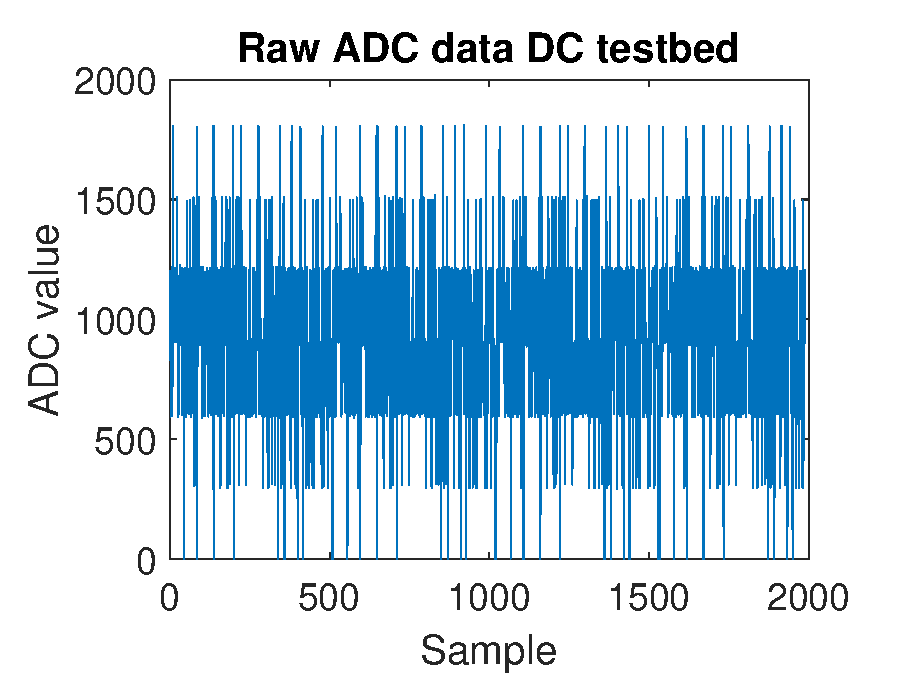
\includegraphics[width=\textwidth]{chapters/evaluation-chapters/hardware/dc/raw-dc-testbed-adc-data-n=9.eps}
    \caption{Raw ADC data from the DC testbed. With seven distinguishable entries, following the on-state of the combinations of LEDs. With a sequence length of 511.}
	\label{fig:raw-dc-testbed-adc-data-n=9}
  \end{minipage}
  \hfill
  \begin{minipage}[b]{0.49\textwidth}
    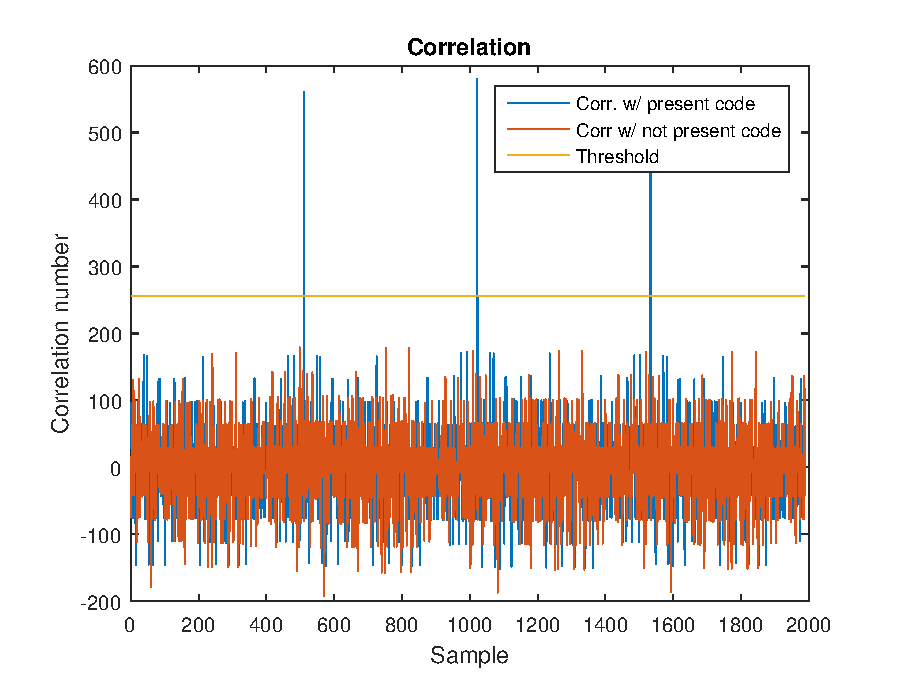
\includegraphics[width=\textwidth]{chapters/evaluation-chapters/hardware/dc/correlation-dc-testbed-n=9.eps}
    \caption{Correlations results from Gold sequences which are and which are not present, with the decision threshold. With a sequence length of 511.}
	\label{fig:correlation-dc-testbed-n=9}
  \end{minipage}
\end{figure}

To show how the F-measure would behave when there are false positives and/or false negatives a different Gold set is chosen.
A length of 127 is chosen, since it may only have three simultaneous continuously modulating LEDs (\autoref{tbl:correlation-gold-families}).
Again the six LEDs are simultaneous continuously modulating with different starting times.
For which the raw ADC can be seen in \autoref{fig:raw-dc-testbed-adc-data-n=7} on the left y-axis and on the right y-axis the current.
And the correlation can be found in \autoref{fig:correlation-dc-testbed-n=7}.
In the correlation figure, peaks can be seen that cross the threshold line, which are the autocorrelation peaks of the sequence.
They are supposed to be there.
But also other results can be seen to cross the threshold line.
These are the false positives, they occur because this code length can not support this much simultaneous transmitters.
The F-measure in time for these correlation results can be found in \autoref{fig:f-measure-dc-testbed-n=7}.
And the precision, recall and F-measure can be found in \autoref{fig:eval-metrics-dc-testbed-n=7}.


\begin{figure}[!tbp]
  \centering
  \begin{minipage}[b]{0.49\textwidth}
    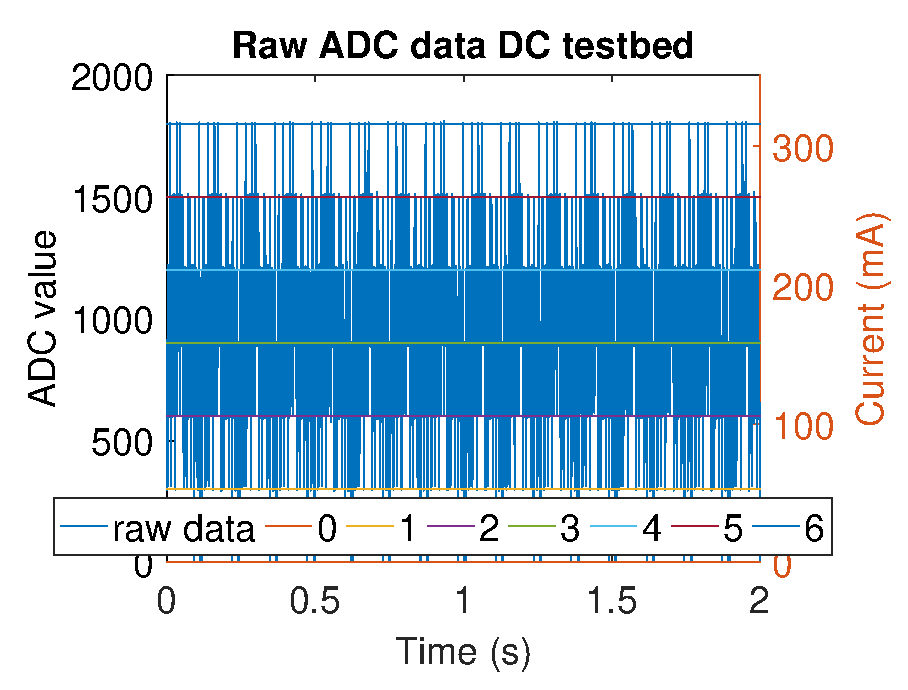
\includegraphics[width=\textwidth]{chapters/evaluation-chapters/hardware/dc/raw-dc-testbed-adc-data-n=7.eps}
    \caption{Raw ADC data from the DC testbed. With seven distinguishable entries, following the on-state of the combinations of LEDs. With a sequence length of 127  on the DC testbed.}
	\label{fig:raw-dc-testbed-adc-data-n=7}
  \end{minipage}
  \hfill
  \begin{minipage}[b]{0.49\textwidth}
    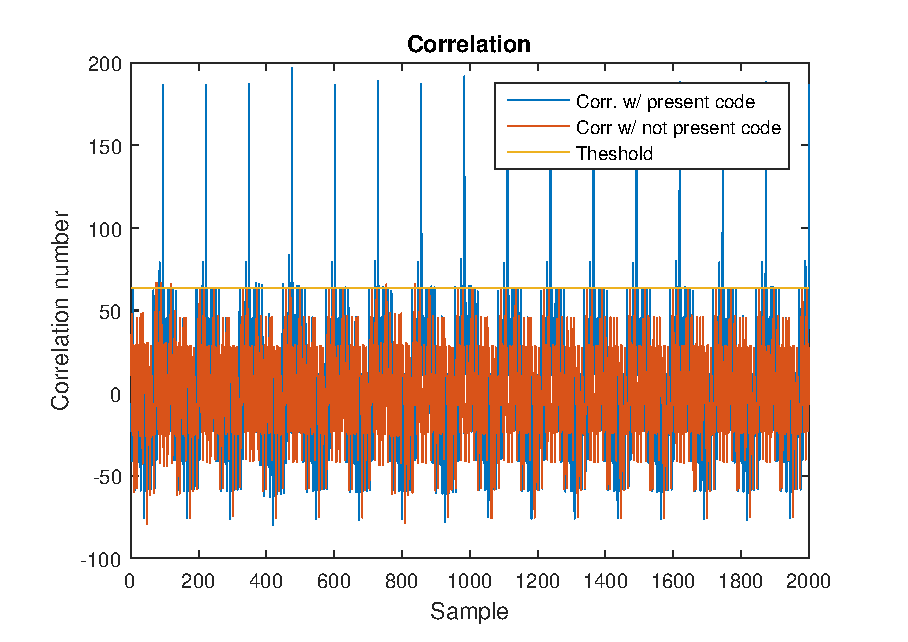
\includegraphics[width=\textwidth]{chapters/evaluation-chapters/hardware/dc/correlation-dc-testbed-n=7.eps}
    \caption{Correlations results from Gold sequences which are and which are not present, with the decision threshold. With a sequence length of 127 on the DC testbed.}
	\label{fig:correlation-dc-testbed-n=7}
  \end{minipage}
\end{figure}


\begin{figure}[!tbp]
  \centering
  \begin{minipage}[b]{0.49\textwidth}
  	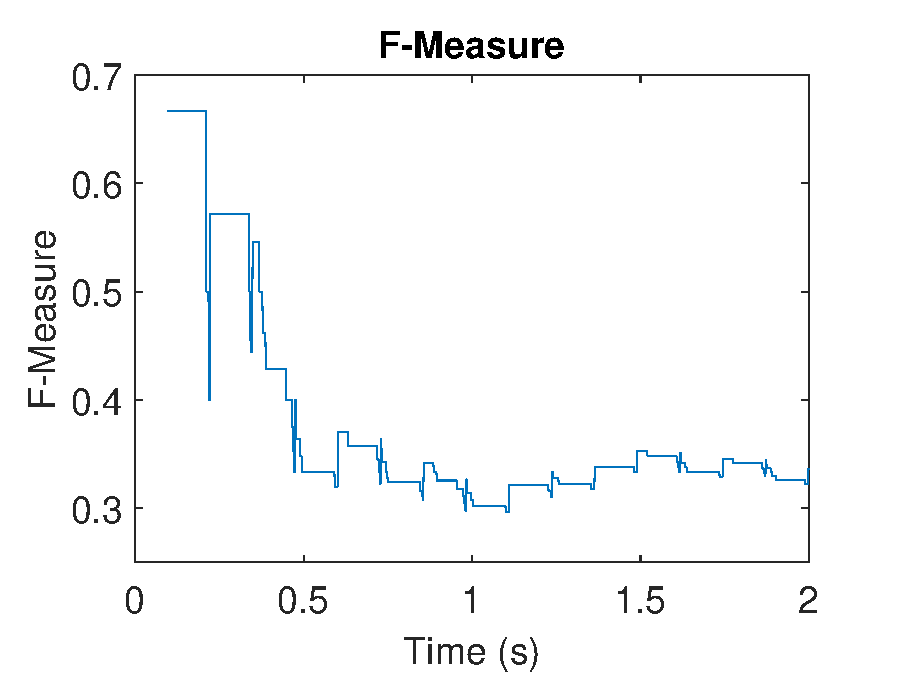
\includegraphics[width=\textwidth]{chapters/evaluation-chapters/hardware/dc/f-measure-dc-testbed-n=7.eps}
  	\caption{F-Measure of DC testbed correlation (\autoref{fig:correlation-dc-testbed-n=7}), with sequence length of 127.}
  	\label{fig:f-measure-dc-testbed-n=7}
  \end{minipage}
  \hfill
  \begin{minipage}[b]{0.49\textwidth}
    \includegraphics[width=\textwidth]{chapters/evaluation-chapters/hardware/dc/eval-metrics-dc-testbed-n=7.eps}
    \caption{Evaluation metrics of DC testbed correlation (\autoref{fig:correlation-dc-testbed-n=7}), with sequence length of 127.}
    \label{fig:eval-metrics-dc-testbed-n=7}
  \end{minipage}
\end{figure}

% !TeX root = ../../../../thesis.tex

\subsection{AC}